\chapter{Introduction}

Application Programming Interfaces, commonly known as APIs, are used to express a software component in terms of its operations, inputs, outputs, and their types\footnote{\url{https://en.wikipedia.org/wiki/Application_programming_interface}}. Robillard defines an API as follows: An API is the interface to implement functionality that developers can access to perform various tasks \cite{Robillard_a_field_study, Robillard_what_makes}. APIs enable multiple software components to interact with each other. Web APIs allow software-to-software interconnectivity using web technologies as the transport mechanism between systems.

REST APIs are a type of API that are used to integrate software components using web technologies. Fielding defined Representational State Transfer or REST as an architectural style for developing distributed hypermedia systems \cite{Fielding_rest}. Fielding described the design of the modern Web as an example of a REST-style architecture. REST-style architecture allows software components to satisfy the data transfer needs of the modern Internet-scale applications by leveraging a generic interface based on URIs and Internet media types that allow intemediate processing such as caching to improve system performance.

The overarching goal of my research is to improve the current state of the REST API documentation process by automating the repeating manual steps. REST APIs allow access to application resources over HTTP. While REST describes a generic protocol for accessing application resources, the applications are responsible for the specific representation of the resources. For example, a REST API may support multiple Internet media types such as JSON, XML, CSV for a single application resource. Similarly, two different REST APIs may use the same media type but contain entirely different formats to represent their objects.

For example, GitHub, an online code repository hosting tool, has a REST API that can be used by third-party applications to integrate with GitHub features. The GitHub REST API\footnote{\url{https://developer.github.com/v3/repos/\#create}} has a resource called \texttt{Repository} to denote a code repository that can be identified by the URL \url{/user/repos}. To create a new \texttt{Repository} for a user, the GitHub API can be invoked via HTTP $POST$ at \url{/user/repos} using the following JSON representation of a \texttt{Repository}:


\begin{verbatim}
{
  "name": "Hello-World",
  "description": "This is your first repository",
  "homepage": "https://github.com",
  "private": false,
  "has_issues": true,
  "has_wiki": true,
  "has_downloads": true
}
\end{verbatim}

In today's world of technology, REST APIs have become ubiquitous and the primary choice for integrating Internet enabled applications due to its simplicity and similarity with HTTP \cite{mangler2010origin}. For example, a real estate listing website uses a REST API to collect ``walk score'' and another REST API to show a map view of a property listing. By incorporating the map and walk score using REST APIs, the real estate listing site provides important information to their users. Most REST APIs, including these two examples, are often documented manually or using custom implemented tools specific to the APIs that are not publicly available. This requires effort to generate and maintain the documentation of REST APIs over time since there is a lack of reusable tool support.

Previous research in the area of API usability mostly focused on local APIs such as Java libraries. Researchers identified the documentation of APIs as both the primary source of information as well as the key obstacle for API usability \cite{Robillard_what_makes}. Hence the quality of the API documentation plays an important role in API usability. To this regard, researchers have identified the qualities of ``good API documentation'' as follows: complete, correct, includes thorough explanations and code examples, provides consistent presentation and organization \cite{Robillard_what_makes,Myers_study}. Today, there are several tools such as Javadoc\footnote{\url{http://www.oracle.com/technetwork/java/javase/documentation/index-jsp-135444.html}}, UsETeC \cite{zhu2014mining}, Jadeite \cite{Jadeite}, APIMiner \cite{montandon2013documenting}, Roast \cite{Hoffman_api_documentation} that can be used to document local APIs with the aforementioned qualities.

While there are overlaps between the documentation requirements of local and REST APIs, there are significant requirements that are unique to each. The differences between the documentation
of local vs. REST APIs can be depicted by an example as follows:
\newcommand*{\captionsource}[2]{%
  \caption[{#1}]{%
    \textbf{Source:} #2%
    \\\hspace{\linewidth}%
    #1%
  }%
}
\begin{figure}[htb]
  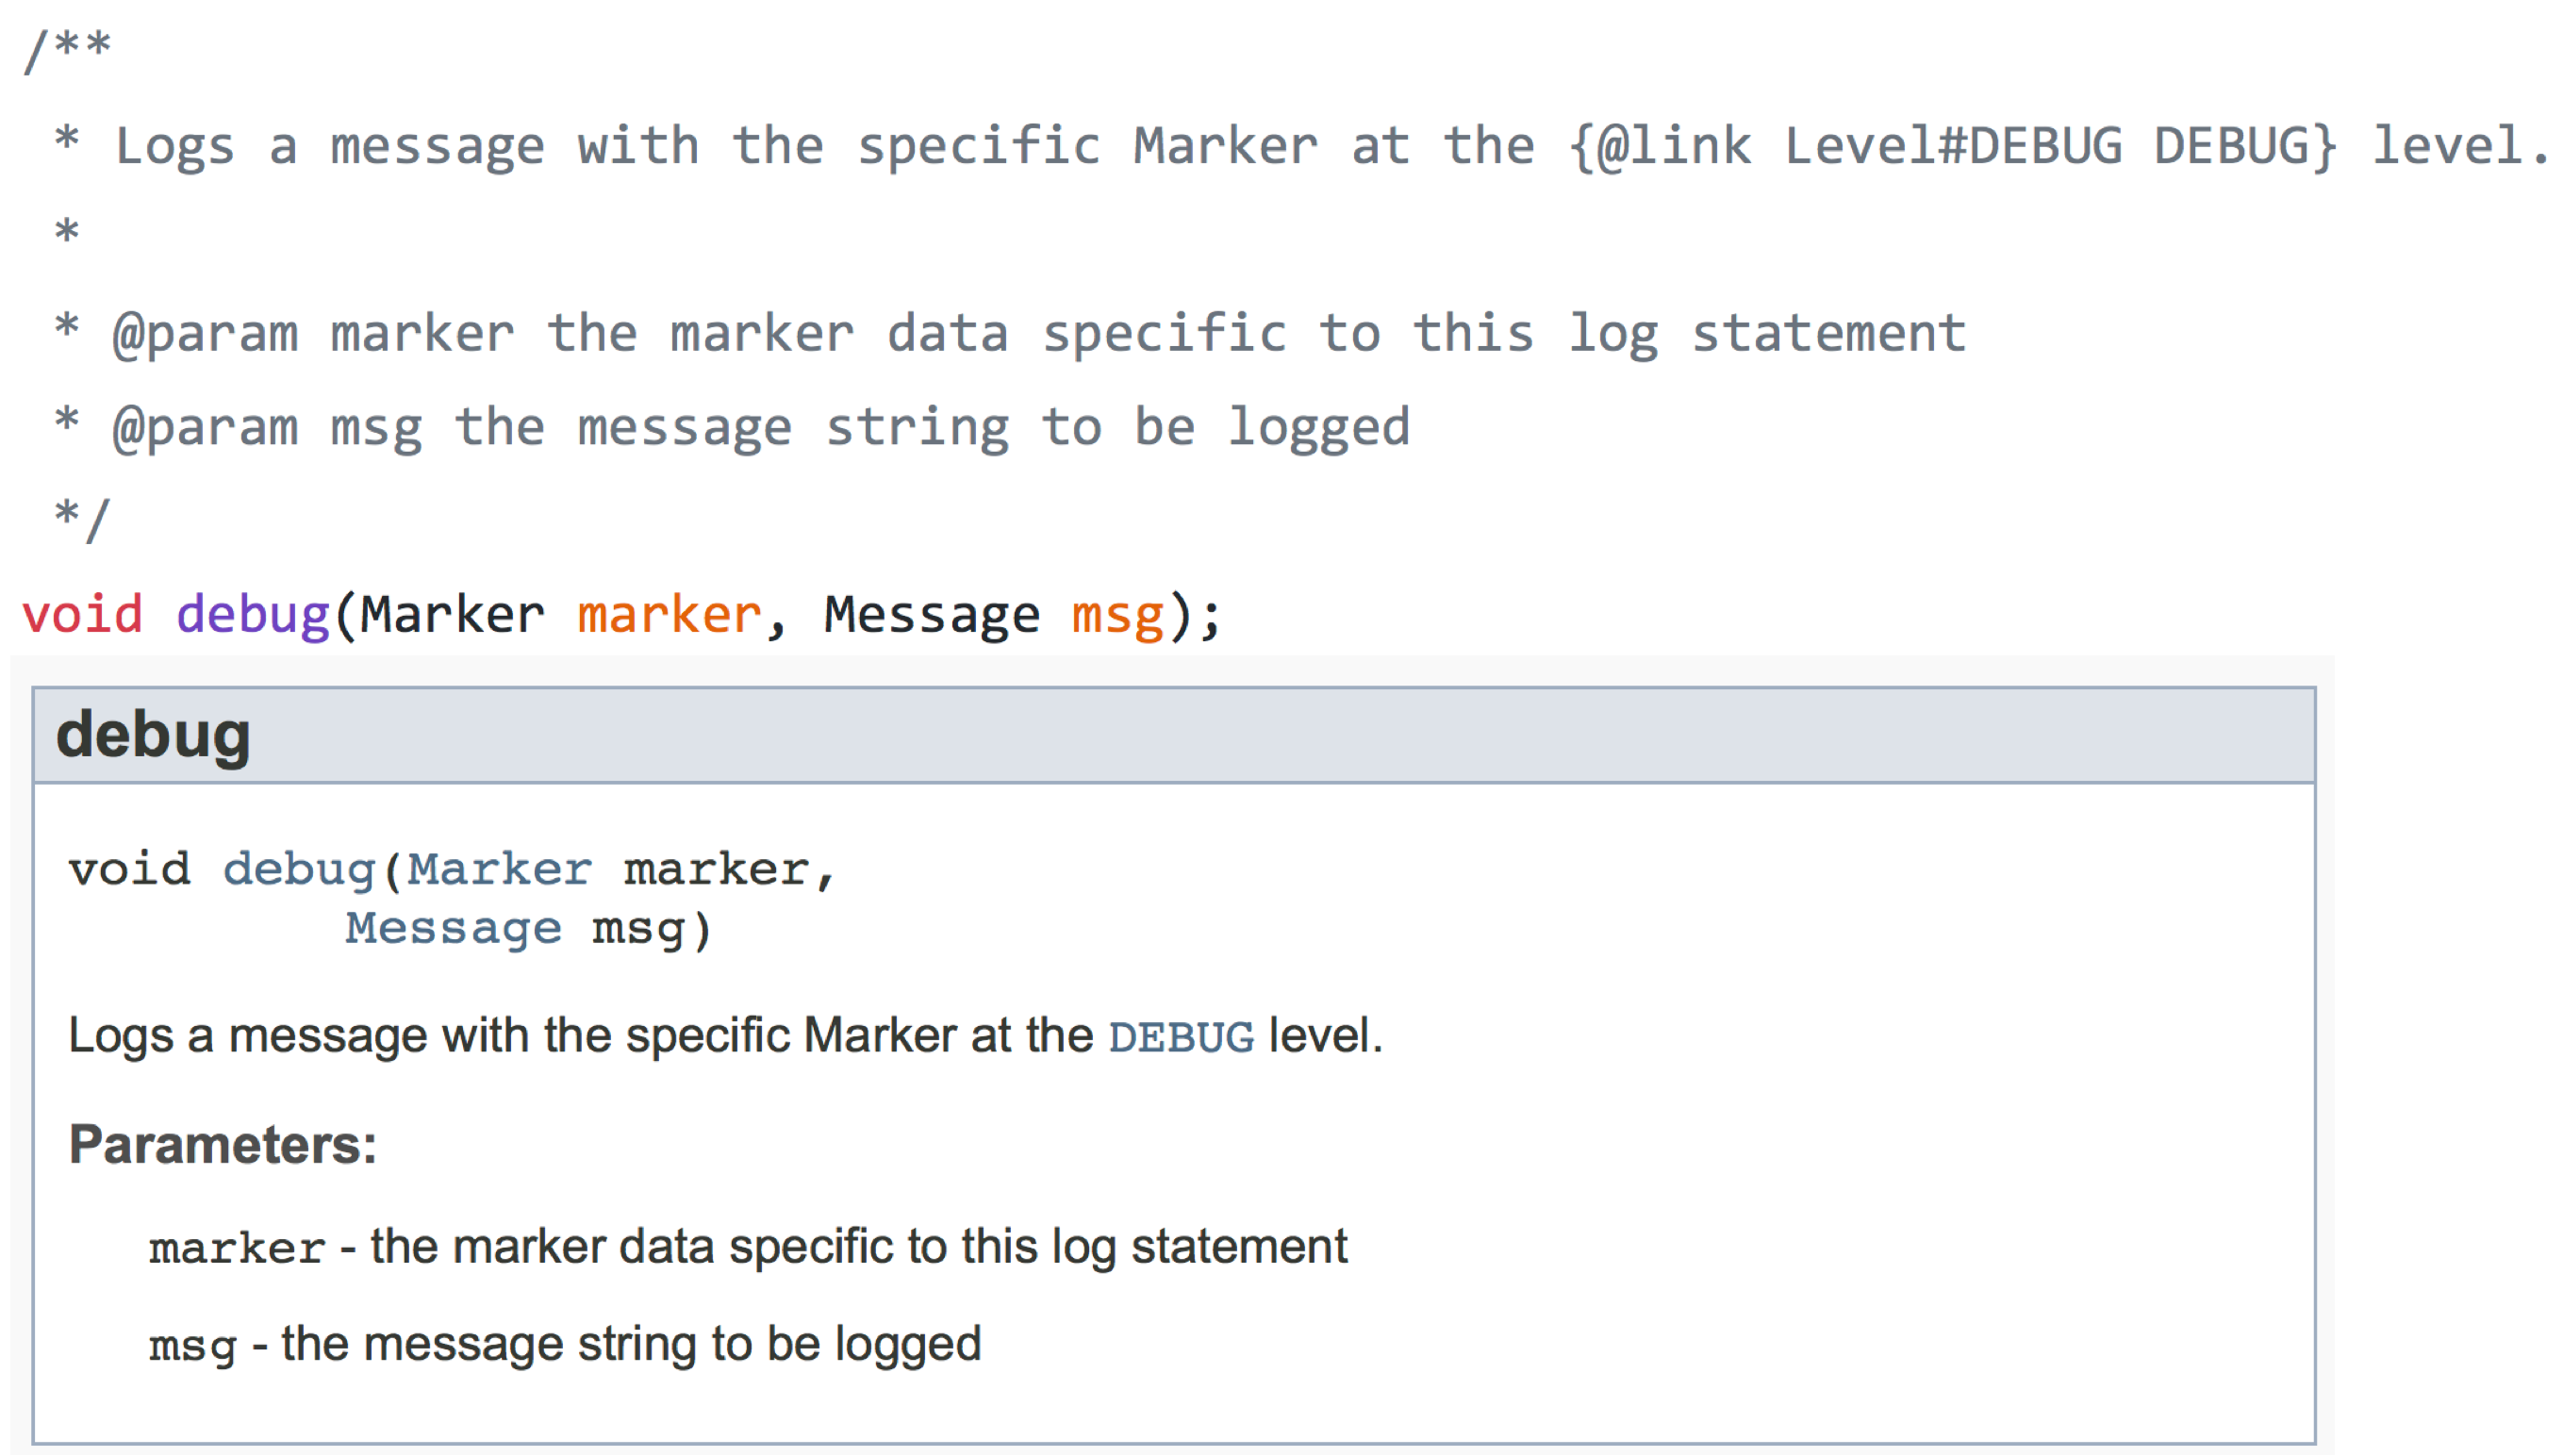
\includegraphics[width=\linewidth]{javadoc.png}
  \captionsource{Example Local API Documentation from Formatted Comments Using JavaDoc}{Log4J}
  \label{fig:javadoc}
\end{figure}



Figure~\ref{fig:javadoc} shows an example of how JavaDoc is used to automatically extract formatted comments from the API source code to
generate human readable documentation. Here the developers of the \texttt{debug} API method provided comments describing the intended way to use the method. JavaDoc can
automatically parse such comments to render the API documentation. Since the comments are not executable code, the API developers need to ensure the correctness of the
comments, and maintain it manually when the API evolves.

\begin{figure}[htb]
  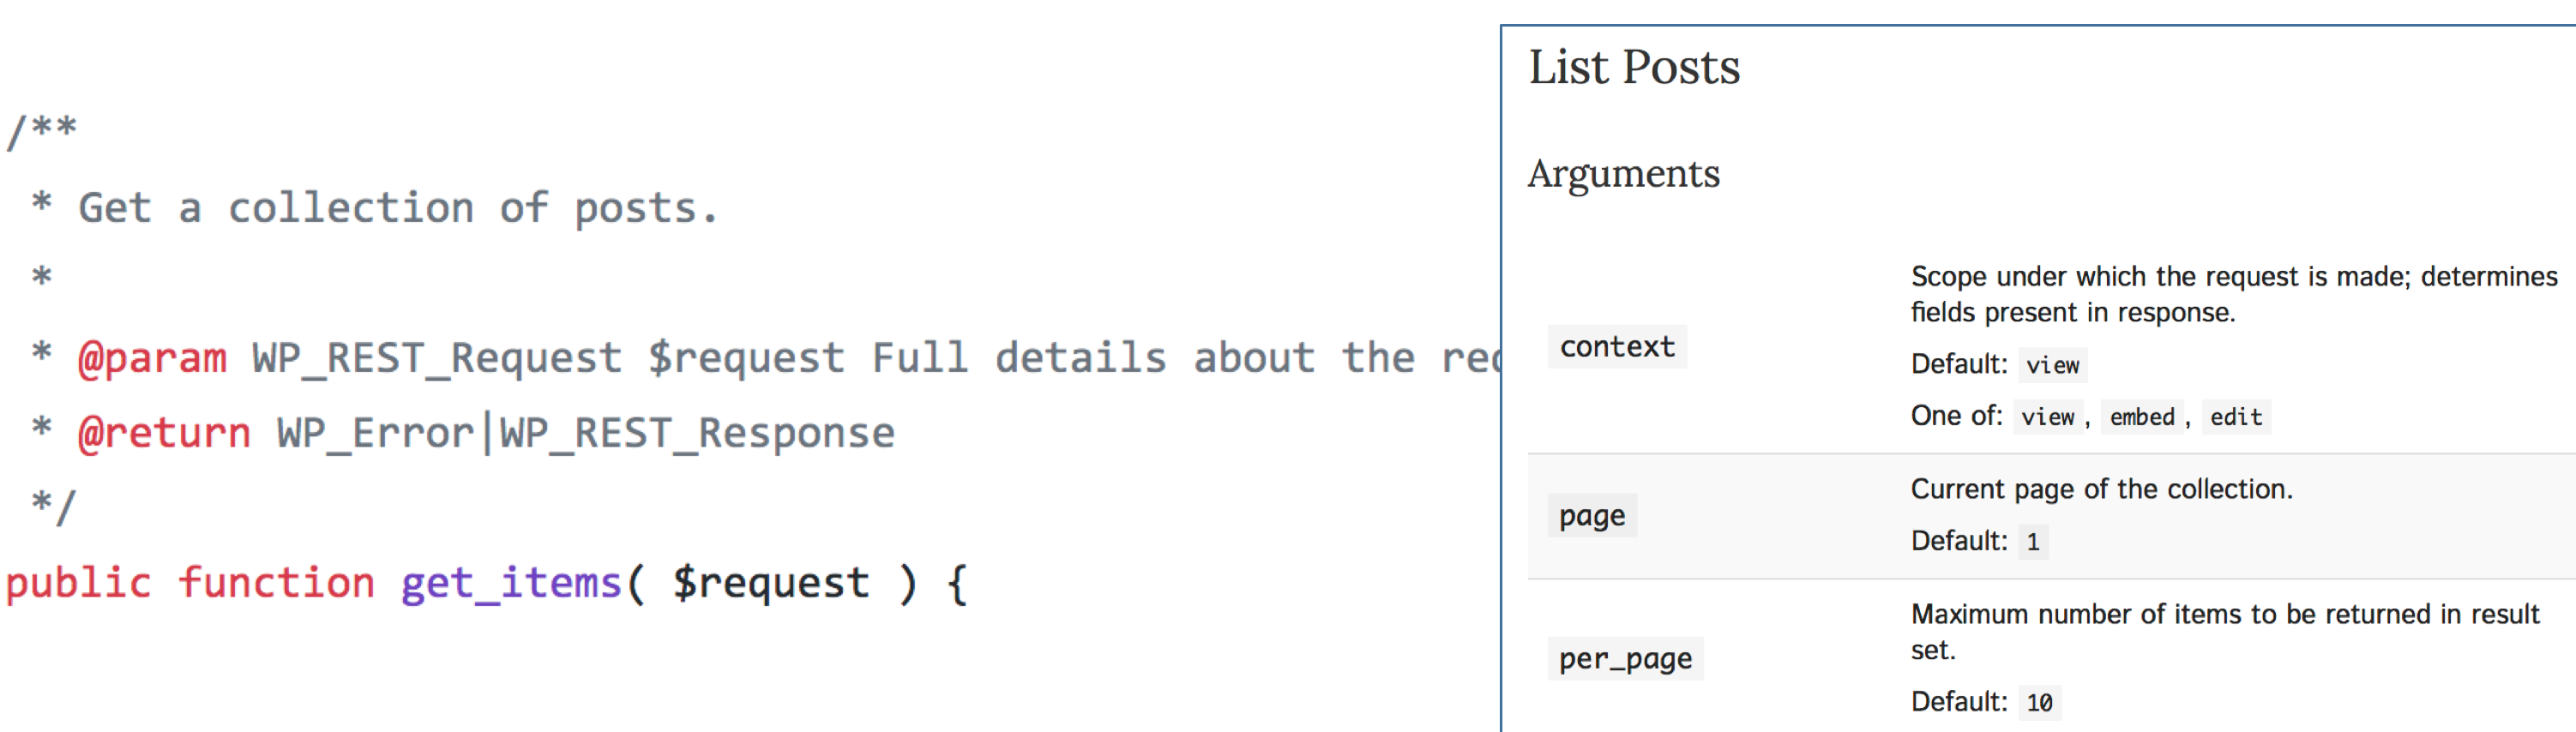
\includegraphics[width=\linewidth]{wordpress_doc.png}
  \captionsource{Difference between a REST API Code and its Documentation}{WordPress REST API}
  \label{fig:wordpress_doc}
\end{figure}


Figure~\ref{fig:wordpress_doc} shows an example of a REST API source code and a fragment of its API documentation
taken from WordPress REST API. The developers of the \texttt{get\_items} API provided formatted comments to describe the intended use of this method similar to the example
in Figure~\ref{fig:javadoc}. However, there is a stark difference between the API source code and its documentation. This is because even though the API is implemented
using a specific language, PHP in this case, the documentation is agnostic to this choice of technology because REST APIs are described by their HTTP interface elements such as
HTTP headers, URLs, and body. As shown in this example, using existing local API documentaiton tools such as JavaDoc that converts formatted comments into API documentation would require extensive
manuall effort for REST APIs for its verbosity and difference between the source code and the documentation constructs.

The documentation of most local APIs
contain a structural definition of the API classes and methods. API usage examples for local APIs are documented using the same programming language of the API. On the other hand, REST APIs
are defined using HTTP specific parameters such as API endpoints, query parameters, HTTP headers and body. REST API clients can be written in any programming language agnostic to the API
implementation language. Due to such structural and implementation differences between local and REST APIs, the existing technique and tools for local API documentation cannot be readily
used to generate REST API documentation.


\begin{figure}[htb]
  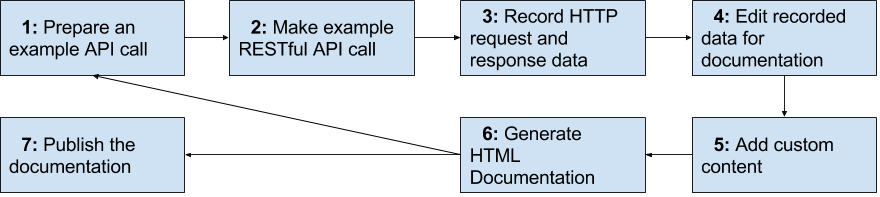
\includegraphics[width=\linewidth]{manual_workflow.png}
  \caption{Manual REST API Documentation Steps}
  \label{fig:manual}
\end{figure}

Currently, the process of documenting REST APIs is largely manual. This is problematic because, it is time a consuming and an error-prone process. Conceptually, the high level steps involved in the manual process can be identified as shown in Figure \ref{fig:manual}. These steps 1-7 can be described as follows:

\begin{enumerate}
  \item API developer prepares an example API with the required HTTP parameters and request body.
  \item API developer uses a REST API client to make the example API call.
  \item the API developer records the HTTP data.
  \item API developer then edits the recorded data so that only relevant content is selected for documentation.
  \item API developers use any custom content to describe the API example.
  \item API developers combine the custom content with the edited content from the HTTP traffic into HTML to publish on the web.
  \item API developer adds custom overview information to explain API concepts and general rules, and publishes the final documentation so other developers can learn the API.
\end{enumerate}

The steps 1-6 are repeated for every API action that needs to be documented, and steps 1-7 need to repeated for every version of the REST API as it evolves. As depicted here, this manual process can be both time consuming and error-prone.

\section{Research Goals}
The principal goal of my research is to improve the REST API documentation process by automating the repeating manual steps in the aforementioned workflow. More specifically, I aim to solve the following research goals:

\begin{itemize}
  \item \textit{RG1: To identify a set of REST API documentation requirements.} Existing research on API usability has derived a number of API documentation requirements primarily focusing on local APIs. Due to the structural and implementation differences between local and REST APIs, I aim to identity REST API specific documentation requirements in my research. This has several implications as follows: having access to a scientifically derived list of REST API documentation requirements allows REST API developers to make an informed decision related to planning and execution of their documentation efforts. The requirements provide a background research that can be used by practitioners to compare and contrast existing REST API documentation tools while selecting an appropriate tool for their API. REST API documentation tool developers can also use the requirements to build necessary features.
  \item \textit{RG2: To develop and evaluate a documentation technique to overcome the commonly observed challenges related to REST API documentation.} I aim to devise a reusable technique so that REST APIs can be documented following the identified REST API documentation requirements without following manual or bespoke methods. It has the following implications: REST API developers can utilize the technique to overcome the common challenges with the generation and maintenance of their API documentation, and REST API client developers can access an API documentation.

\end{itemize}


\section{Research Questions}
Related to RG1 and RG2, I aim to address the following research questions as my objectives:

\begin{itemize}
  \item \textit{RQ1: How are evolving REST APIs documented?} This question is aimed to analyze the gap between current industry practice around the documentation of evolving REST APIs and the propose solutions from existing literature. This objective helped me to identify the research opportunity to work on unresolved problems related to REST API documentation.
  \item \textit{RQ2: What are the requirements for usable REST API documentation?} Answer of this question provides a necessary background for improving the state of REST API documentation process.
  \item \textit{RQ3: What technique can be used to document REST APIs to meet the requirements?} This is the central research question. I researched to develop a new technique that can fill the gap between existing REST API documentation methods and the identified requirements.
  \item \textit{RQ4: Is the proposed technique practical for REST API developers?} A qualitative evaluation of the proposed technique in a real-world setup is needed to understand the feasibility and the shortcomings of the proposed technique from the perspective of the REST API developers.
  \item \textit{RQ5: How does documentation using the proposed technique impact REST API client developers?} This question investigates the impact of the proposed technique from the perspective of the REST API client developer effort and success rate while performing API tasks.
\end{itemize}

\section{Cohesion and Unitary Report}
To address the aforementioned research goals and objectives, my research strategy included five sub-projects, which have resulted in publications at peer-reviewed international conferences. Table~\ref{table:chapter_summary} shows a high level overview of the flow of arguments between the sub-projects to meet the research goals and questions.

\begin{table}
  \caption{Summary and Flow of Arguments of the Sub-projects}
  \begin{tabular}{|p{1.5cm}|p{1.5cm}|p{1.5cm}|p{4.5cm}|p{6cm}|}
  \hline
  Chapter & Goal & Question& Research Project & Primary Outcome \\
  \hline
  Chapter~\ref{chapter:case_study}  & RG1 & RQ1 & A case study of Web API evolution \cite{sohan2015case}. & A set of challenging problems related to evolving Web APIs. Selected REST API documentation as the problem of interest for this research. \\
  \hline
  Chapter~\ref{chapter:spy_rest} & RG1 and RG2 & RQ2 and RQ3 & SpyREST: Automated RESTful API documentation using an HTTP proxy server \cite{sohan2015spyrest}. & A list of requirements. A conceptual design using interception to generate REST API documentation to meet the requirements. \\
  \hline
  Chapter~\ref{chapter:demo_paper} & RG2 & RQ3 & SpyREST in action: An automated RESTful API documentation tool \cite{sohan2015spyrest_tool}. & A reusable tool that implements the conceptual design and shows how the identified REST API documentation requirements are met.\\
  \hline
  Chapter~\ref{chapter:cisco_study} & RG2 & RQ4 & Automated example oriented REST API documentation at Cisco \cite{sohan_cisco}. & Empirical evidence that the proposed technique provides a practical documentation solution for REST API developers.\\
  \hline
  Chapter~\ref{chapter:controlled_study} & RG2 & RQ5 & A study of the effectiveness of usage examples in REST API documentation \cite{sohan_vlhcc}. & Empirical evidence that the proposed technique allows REST API client developers to perform API tasks with less effort, higher success and satisfaction ratings.\\
  \hline
\end{tabular}
\label{table:chapter_summary}
\end{table}

The first research project is described in Chapter~\ref{chapter:case_study}, where I discuss a case study to summarize the state of existing literature and industry practices related to the versioning, documentation, and change communication patterns of evolving Web APIs \cite{sohan2015case}. The results are based on a study of nine industrial APIs. I found a lack of reusable techniques in the existing literature to automatically generate and maintain the documentation of multi-version evolving REST APIs with usage examples. I pursued further research to solve this problem as discussed in the following paragraphs.

In Chapter~\ref{chapter:spy_rest}, I discuss my second research project where I derived a set of REST API documentation requirements and proposed a new technique to meet the requirements \cite{sohan2015spyrest}. Here, I present a list of REST API documentation requirements by studying the literature and applying the findings from Chapter~\ref{chapter:case_study}. I discuss the available REST API documentation techniques and compare against the requirements. I present, \textit{SpyREST}, a novel technique to intercept example REST API calls using an HTTP proxy server to collect and automatically synthesize API traffic to generate and update API documentation to satisfy the identified requirements. The primary advantage of the presented technique is that the documentation is generated from executable code. As a result, a continuously updated REST API documentation with realistic usage examples is achievable with a reduced manual effort. The remaining chapters provide evidence that the proposed technique can satisfy the identified requirements.

I present my third research project, related to RG2, in Chapter~\ref{chapter:demo_paper}, where I present a prototype implementation of the aforementioned technique \cite{sohan2015spyrest_tool}. In this prototype implementation, I discuss the process that transforms a number of example HTTP requests and responses into usable REST API documentation. I also present an example where automated test code is used to generate and maintain a continuously updated REST API documentation using the developed tool.

I discuss my fourth research project, related to RG2, involving an industrial evaluation of the proposed technique and the tool in Chapter~\ref{chapter:cisco_study} \cite{sohan_cisco}. The evaluation is carried out based on the data collected from an 18 month production use of SpyREST at Cisco, my current employer. From the study I found that it is effective to use the proposed interception technique and automated tests to document evolving REST APIs satisfying the previously presented REST API documentation requirements. Automated always-updated REST API documentation was found to help establish a quick feedback cycle among the stakeholders. I also discuss several refinements and limitations of the proposed technique based on the lessons learned from this case study.

I present my fifth research project, related to RG2, in Chapter~\ref{chapter:controlled_study}, where I discuss a controlled study to understand the impact of usage examples in API documentation on REST API client developers \cite{sohan_vlhcc}. I observed that providing usage examples with data taken from API test code reduces the obstacles and improves API client developer success rate, reduces required trial attempts, and improves satisfaction ratings. The findings from this study provides an empirical evidence that by using the proposed technique of generating REST API documentation from API test code can help API client developers to achieve a higher level of success with a reduced effort.

In Chapter~\ref{chapter:conclusion}, I conclude by discussing how the research objectives are achieved and provide a list of potential future research problems.

\section{Contributions}
In summary, this thesis makes the following key contributions to the body of research in software engineering:


\begin{enumerate}
  \item A list of REST API documentation requirements derived from the existing literature and the current state of industry practices to be used as a guideline by practitioners and researchers.
  \item SpyREST, a novel technique and a reusable tool that uses interception to automatically generate and maintain evolving REST API documentation with usage examples from executable code.
  \item An industrial evaluation of SpyREST to demonstrate the feasibility of the proposed technique that REST API developers can follow to improve their REST API documentation experience.
  \item An empirical evidence showing the common obstacles faced by REST API client developers that can be reduced with usage examples to help the prioritization of REST API documentation efforts.
\end{enumerate}

\newpage
\bibliographystyle{IEEEtran}
\bibliography{IEEEabrv,references}


